\documentclass{article}

% NeurIPS 2024, camera-ready (final shows author names)
\usepackage[final]{neurips_2024}

\usepackage[utf8]{inputenc}
\usepackage[T1]{fontenc}
\usepackage{hyperref}
\usepackage{url}
\usepackage{booktabs}
\usepackage{amsfonts}
\usepackage{amsmath,amssymb}
\usepackage{nicefrac}
\usepackage{microtype}
\usepackage{graphicx}
\microtypesetup{expansion=false,protrusion=false}

\title{Priority-Conditioned Retention: A Controllable\\
Middle-Layer Memory Circuit in Pretrained Mamba}

\author{%
  Chanhee Jeong \quad Yejun Ahn \quad Suyun Kim \\[3pt]
  Applied Artificial Intelligence, Sungkyunkwan University \\
  Seoul, Republic of Korea
}

\begin{document}

\maketitle

\begin{abstract}
State-space models (SSMs) such as Mamba compress an entire history into a
fixed-size continuous hidden state, achieving linear-time inference at the cost
of associative recall: unlike attention, they cannot losslessly retrieve an
arbitrary past token. Prior work attributes this to a capacity bound but leaves
open whether the practical failure is a \emph{storage} limit or a \emph{control}
limit. We show that a pretrained Mamba-790m already contains a controllable,
spatially localized memory circuit, accessible at inference with no fine-tuning.
By scaling the pre-softplus input to the $\Delta$ gate at positions downstream of
a target, we reduce the effective decay applied to that target and recover
associative recall on a capacity-pressured multi-query associative-recall (MQAR)
task ($0.53 \to 0.73$ at the optimal operating point). The effect is
dose-dependent, target-specific, and bidirectional, and it is localized to a
middle-layer band. Fine-grained ablation identifies a minimal 4-layer core at
L19--22 that matches the 8-layer result ($0.70$ vs.\ $0.67$, equal within noise
at $n{=}150$) at nearly identical perplexity cost ($\times 1.08$ vs.\ $\times 1.07$), whereas the
all-layer intervention inflates perplexity $\times 1.81$. We frame
this as the continuous-state analogue of importance-aware KV-cache compression
and report a boundary: a literal write-quantization analogue does
\emph{not} transfer, because the superimposed state has no per-item slots to
reallocate.
\end{abstract}

\section{Introduction}
Mamba and related selective SSMs match Transformers on many language tasks while
running in linear time, but remain markedly weaker at \emph{associative recall}
--- retrieving a specific value bound to a key seen earlier in context.
\citet{jelassi2024} show this stems from a fundamental capacity constraint: a
fixed state cannot losslessly copy arbitrarily long inputs. Yet a capacity bound
does not, by itself, explain \emph{behavioral} recall failure at moderate load.
The failure could be (a) a \textbf{control} problem (the recurrence applies a
default recency decay and does not preferentially keep query-relevant items),
or (b) a \textbf{storage} problem (the state is genuinely out of bits). These
have opposite implications: (a) is fixable at inference; (b) is not.

This paper provides evidence for (a) in a regime where it matters. We do
\emph{not} modify or retrain the model. Instead we ask: does a pretrained Mamba
already expose a handle that lets us trade its default recency policy for a
target-preserving one? We find that it does, that the handle is the $\Delta$
gate, and, most importantly, that the handle is localized to a contiguous
band of middle layers. Operating only on that band recovers recall at almost no
cost in language-modeling quality, the behavior one expects of a localized
mechanism rather than a diffuse one.

\paragraph{Contributions.}
\begin{itemize}
\item A test-time intervention on the $\Delta$ gate that controllably preserves a
target item in a capacity-pressured SSM, with dose-response, specificity, and
bidirectionality controls (Section~\ref{sec:control}).
\item Localization of this control to layers~16--23 of Mamba-790m, and a
\emph{surgical} result: the 8-layer intervention matches most of the full-model
recall gain at perplexity $\times 1.07$ vs.\ $\times 1.81$
(Section~\ref{sec:circuit}). Fine-grained ablation further identifies a 4-layer
minimal circuit (L19--22) that matches the 8-layer recall ($0.70$ vs.\ $0.67$;
confirmed equivalent at $n{=}150$, Experiment~F) at $\times 1.08$ cost,
and is both sufficient and necessary within L16--23 (Experiment~G).
\item A framing placing this control on a single axis with importance-aware
KV-cache compression, plus a negative result: a literal
write-quantization analogue fails, bounding how far the cache analogy carries
(Section~\ref{sec:boundary}).
\end{itemize}
On scope: all positive results are for Mamba-790m on synthetic
MQAR. We observe non-replication on Mamba-1.4b and fragility on natural language
(Section~\ref{sec:limits}).

\section{Background and Framing}
\paragraph{The $\Delta$ gate as a retention knob.}
In a selective SSM the state updates as
$h_t = \bar{A}_t h_{t-1} + \bar{B}_t x_t$, with $\bar{A}_t = \exp(\Delta_t A)$ and
$A<0$, so $\Delta_t>0 \Rightarrow \bar{A}_t \in (0,1)$. The contribution of token
$i$ surviving to a query at position $T$ is therefore
$\bar{B}_i x_i \cdot \prod_{\tau>i}\bar{A}_\tau$. Two facts follow. First, the
default policy is recency-biased: older contributions decay geometrically.
Second, the \emph{survival} of an item is governed by the \emph{downstream}
decays $\prod_{\tau>i}\bar{A}_\tau$, not by the item's own write alone. Reducing
$\Delta$ at positions after a target pushes those $\bar{A}_\tau \to 1$, slowing
the decay the target experiences --- a preservation lever requiring no weight
change.

\paragraph{Discrete $\leftrightarrow$ continuous importance allocation.}
The KV-cache compression literature
\citep{kivi,kvquant,zipcache,turboquant} implements one principle: spend more
bits on more important tokens. This presumes a slotted cache with random access.
Mamba has no slots --- all items are superimposed in one vector. We therefore
treat ``importance $\to$ retained information'' as architecture-agnostic and
instantiate it in Mamba not as per-token bit allocation but as \emph{differential
retention} through the $\Delta$ gate. We name this framing Priority-Conditioned
Retention (PCR). Section~\ref{sec:boundary} reports where the analogy holds and
breaks.

\section{Method}
\paragraph{Task.}
Multi-query associative recall (MQAR) with random single-token key/value words
(no semantic priors). A prompt presents $N$ key--value pairs followed by a query
key; the model must emit the bound value. Capacity pressure is induced by
increasing $N$; we query the first pair as the default target. As $N$ grows the
base model degrades smoothly (recall $0.77 \to 0.53 \to 0.40$ for
$N{=}16,32,64$); we adopt $N{=}32$ (base recall $0.53$) as the operating point
that balances pressure and headroom.

\paragraph{Intervention.}
We register forward hooks on each layer's \texttt{dt\_proj} and multiply its
pre-softplus output by a per-position gain $g$. Setting $g<1$ (``other-gain'') at
positions downstream of the target's value reduces their effective decay. A layer
mask restricts the intervention to a chosen subset of layers. The model runs on
its pure-PyTorch sequential path (fused kernels intentionally not installed) so
the $\Delta$ pathway is hookable. No parameters are updated.

\paragraph{Model and metrics.}
\texttt{state-spaces/mamba-790m-hf} (48 layers, fp32). We report top-1 recall
over 30 random seeds per condition, and perplexity on a fixed held-out passage
under the same gain, relative to the unmodified model.

\section{Results}
\subsection{Test-time control}\label{sec:control}
Sweeping other-gain at $N{=}32$ over all layers yields a clear inverted-U with an
optimum at $g{=}0.8$, where recall rises $0.53 \to 0.73$, then collapses for
$g \le 0.6$ as integration halts (Figure~\ref{fig:dose}). The non-monotonicity is
mechanistically expected: lowering $\Delta$ both slows decay
($\bar{A}_\tau\to 1$, helpful) and shrinks the write
$\bar{B}_\tau=\Delta_\tau B_\tau$ (harmful); past $g\approx 0.7$ the latter
dominates and integration stalls.

\begin{figure}[t]
  \centering
  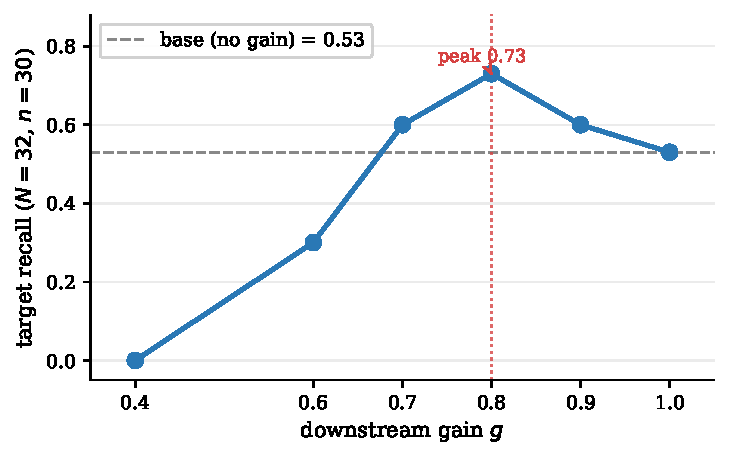
\includegraphics[width=0.62\linewidth]{nfig_dose.pdf}
  \caption{Dose--response of the $\Delta$-gate intervention (Mamba-790m,
  MQAR $N{=}32$). Recall peaks at $g{=}0.8$ ($0.53\to0.73$) and collapses when
  $\Delta$ is over-suppressed, confirming $\Delta$ as a graded retention knob.}
  \label{fig:dose}
\end{figure}

The effect is \textbf{target-specific}: applying $g{=}0.8$ to downstream
positions yields $0.73$, whereas the same gain budget on \emph{random} positions
yields only $0.50$ (near base), ruling out a generic ``more gain helps'' artifact
(Table~\ref{tab:control}). It is also \textbf{bidirectional}: \emph{increasing}
$\Delta$ degrades recall below base, so the sign of the intervention maps to the
sign of the effect.

\begin{table}[t]
\centering
\caption{Specificity and direction controls at $N{=}32$, $g{=}0.8$
(base recall $0.53$). Only targeted downstream suppression helps.}
\label{tab:control}
\begin{tabular}{lc}
\toprule
Condition & Target recall \\
\midrule
Base (no intervention) & 0.53 \\
\textbf{Downstream suppression} ($g{=}0.8$) & \textbf{0.73} \\
Random-position suppression ($g{=}0.8$) & 0.50 \\
Upstream / increase $\Delta$ & $<0.53$ \\
\bottomrule
\end{tabular}
\end{table}

\subsection{Layer localization and the surgical circuit}\label{sec:circuit}
Restricting $g{=}0.8$ to 8-layer bands isolates the responsible depth: recovery
concentrates in \textbf{L16--23} ($+0.13$), with a secondary contribution at
L24--31 ($+0.07$) and nothing elsewhere (Figure~\ref{fig:layers}). Crucially, the
localization is also \emph{cheaper}: Table~\ref{tab:main} shows the 8-layer
intervention captures most of the recall gain at near-zero language-modeling
cost, while the all-layer version pays a large perplexity tax. A targeted edit to
the memory circuit is almost free while a global one is not, which is what we would
expect from a dedicated mechanism rather than a diffuse property.

\begin{figure}[t]
  \centering
  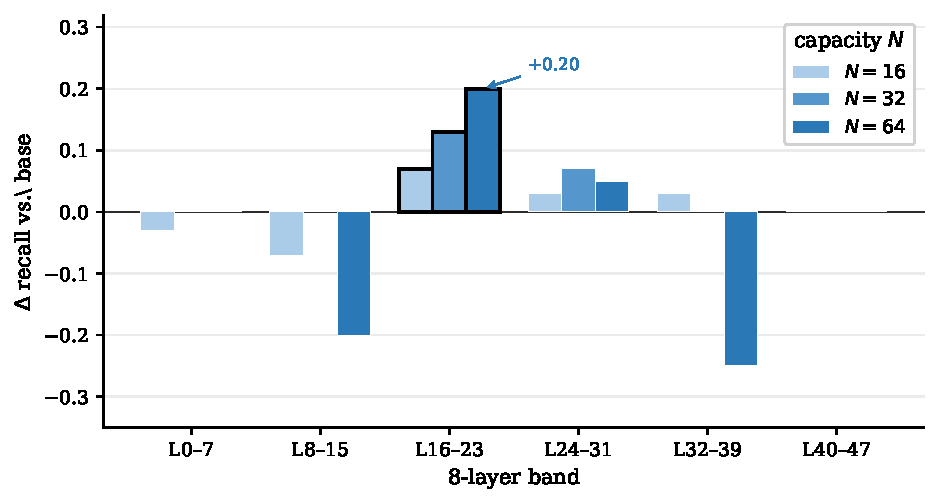
\includegraphics[width=0.62\linewidth]{nfig_layers.pdf}
  \caption{Layer-band localization across capacity levels (Experiment~A). Applying
  $g{=}0.8$ to one 8-layer band at a time, L16--23 is the top band at every $N$.
  At $N{=}64$, off-target bands L8--15 ($-0.20$) and L32--39 ($-0.25$) turn
  actively harmful, making the surgical choice more important under pressure.}
  \label{fig:layers}
\end{figure}

\begin{table}[t]
\centering
\caption{Test-time $\Delta$-gate intervention across capacity levels
(Mamba-790m, $g{=}0.8$, base ppl $\approx 232$; $n{=}30$ for $N\le32$, $n{=}20$ at
$N{=}64$). PPL cost is $N$-independent. L16--23 holds a positive advantage at every
level and overtakes the all-layer intervention at $N{=}64$ ($\mathbf{0.60}>0.55$) as
off-target layers turn harmful; the 4-layer minimal core L19--22 (Section~\ref{sec:circuit})
is strongest at $N{=}32$ but regresses below base at $N{=}64$. The knockout row tests
necessity (L19--22 removed from L16--23).}
\label{tab:main}
\begin{tabular}{lcccc}
\toprule
Intervention & $N{=}16$ & $N{=}32$ & $N{=}64$ & PPL \\
\midrule
Base (no gain)                     & 0.77 & 0.53 & 0.40 & $\times 1.00$ \\
All layers, $g{=}0.8$             & 0.90 & 0.73 & 0.55 & $\times 1.81$ \\
\textbf{L16--23 (8L)}, $g{=}0.8$ & 0.83 & 0.67 & \textbf{0.60} & $\mathbf{\times 1.07}$ \\
L19--22 (4L), $g{=}0.8$          & 0.87 & 0.70 & 0.35 & $\times 1.08$ \\
\midrule
\multicolumn{5}{l}{\textit{Necessity (knockout, $N{=}32$):}} \\
$\{16,17,18,23\}$ (L19--22 removed) & --- & 0.43 & --- & --- \\
\bottomrule
\end{tabular}
\end{table}

To verify that L16--23 is not an artifact of the $N{=}32$ operating point, we
swept the band localization at $N\in\{16,32,64\}$ (Experiment~A). L16--23 is the
top 8-layer band at every pressure level, and its advantage grows with load
(Table~\ref{tab:main}). At $N{=}64$ a notable reversal emerges: the surgical
circuit ($0.60$) overtakes the all-layer intervention ($0.55$). Per-band
inspection shows why: L8--15 and L32--39, neutral at low $N$, shift to $-0.20$
and $-0.25$ at $N{=}64$. Off-target harm grows with capacity pressure and the
surgical variant avoids it entirely. Not only does L16--23 suffice; the
surrounding layers actively interfere under high load.

To identify the minimal effective sub-circuit, we performed a fine-grained
ablation within L16--23 (Experiment~B, $N{=}32$, $g{=}0.8$). Sliding 4-layer
windows across L16--27 show the recall gain is concentrated in the rear of the
band: L19--22 achieves recall $0.70$ ($\Delta{+}0.17$), matching the full 8-layer band
within sampling noise. Earlier windows are weaker
(L16--19: $\Delta{+}0.10$; L17--20, L18--21: $\Delta{+}0.13$), and L23--26 is
actively harmful ($-0.10$). Individual-layer inspection confirms L23 as a boundary
layer ($-0.13$ alone). The 4-layer sub-band L19--22 therefore constitutes a
\emph{minimal effective circuit}: half the layers, nearly identical PPL cost
($\times 1.08$ vs.\ $\times 1.07$), and recall statistically equivalent to the
8-layer band (Table~\ref{tab:ci}, Experiment~F). The surrounding layers L16--18
and L23 dilute rather than contribute. Experiment~G further confirms that L19--22
is not merely sufficient but \emph{necessary}: removing it from L16--23 (leaving
only layers~$\{16,17,18,23\}$) collapses the gain to $\Delta{-}0.10$ below base
(Table~\ref{tab:main}, knockout row).

\paragraph{Robustness and statistical validation (Experiments F--H).}
We re-ran the load-bearing $N{=}32$ comparisons at $n{=}150$ (Table~\ref{tab:ci}):
both circuits lift recall well above base (L16--23 $0.780$, L19--22 $0.773$), and
their 95\% Wilson intervals overlap heavily, so the $0.03$ gap seen at $n{=}30$ is
sampling noise; we characterise L19--22 as \emph{matching} L16--23, not exceeding
it. (The $n{=}150$ base of $0.620$ likewise places the $n{=}30$ estimate of $0.53$
on the low side of its sampling distribution, leaving the intervention deltas
intact.) Across capacity levels the two circuits diverge (Table~\ref{tab:main},
Figure~\ref{fig:layers}): the 4-layer core matches the 8-layer band at $N{\le}32$
but \emph{regresses below base} at $N{=}64$ ($0.35<0.40$), whereas L16--23 stays
positive and reaches its largest advantage there ($+0.20$; a dedicated
$N\in\{8,\dots,64\}$ sweep (Experiment~H) confirms the protected-vs-base gap peaks
at $N{=}64$, $+50\%$ relative). L19--22 is thus the efficient choice at the operating point,
L16--23 the robust choice under sustained pressure.

\begin{table}[t]
\centering
\caption{Statistical validation at $N{=}32$, $g{=}0.8$ ($n{=}150$, 95\% Wilson CI).
The $0.03$ gap between L19--22 and L16--23 at $n{=}30$ falls within noise; both circuits
are equivalent. (Experiment~F)}
\label{tab:ci}
\begin{tabular}{lccc}
\toprule
Condition & Hits/$n$ & Mean & 95\% CI \\
\midrule
Base (no gain)  & 93/150  & 0.620 & $[0.54, 0.69]$ \\
L16--23 (8L)    & 117/150 & 0.780 & $[0.71, 0.84]$ \\
L19--22 (4L)    & 116/150 & 0.773 & $[0.70, 0.83]$ \\
\bottomrule
\end{tabular}
\end{table}

\paragraph{Scale check: Mamba-130m (Experiment~C).}
To assess whether a proportional circuit exists in a smaller model, we applied the
same 4-layer window sweep to Mamba-130m (24 layers, $N{=}32$, $g{=}0.8$). Under
the proportional-depth hypothesis, the 790m circuit at L19--22
(${\approx}40$--$47\%$ depth) would predict a counterpart near L9--11 in 130m.
The result (Table~\ref{tab:scale}) does not support this: the best 4-layer window
is L13--16 ($57$--$70\%$ depth), shifted well downstream of the prediction, and the
peak gain is $\Delta{+}0.06$, less than half the 790m effect. Eleven of 21
windows are actively harmful, and the all-layer intervention degrades both recall
($0.43$, below base $0.57$) and language quality ($\times 1.31$). Notably, L13--16
reduces perplexity ($\times 0.95$), suggesting that $\Delta$ is already elevated
by default in those layers of 130m. Fine-grained ablation within L13--16 finds a
weakly superior 2-layer sub-window (L14--15, $\Delta{+}0.03$), with individual
layers each contributing nothing above base ($\Delta{+}0.00$), indicating no
single-layer concentration. The proportional-depth prediction fails, and the effect
magnitude is substantially reduced. We treat these results as a boundary condition
rather than a positive replication (Section~\ref{sec:limits}).

\begin{table}[t]
\centering
\caption{Scale comparison at $N{=}32$, $g{=}0.8$. The 790m minimal circuit does
not transfer proportionally to 130m: the optimal window shifts deeper, the recall
gain is substantially weaker, and PPL behavior reverses.}
\label{tab:scale}
\begin{tabular}{lccccc}
\toprule
Model & Layers & Best circuit & Depth & $\Delta$ recall & PPL \\
\midrule
Mamba-790m & 48 & L19--22 (4L) & $40$--$47\%$ & $+0.17$ & $\times 1.08$ \\
Mamba-130m & 24 & L13--16 (4L) & $57$--$70\%$ & $+0.06$ & $\times 0.95$ \\
\bottomrule
\end{tabular}
\end{table}

\paragraph{JRT baseline (Experiment~D).}
Just Read Twice (JRT; \citealt{jrt}) is a natural training-free baseline: repeat the
key--value context before the query so the model compresses it a second time, at a
cost of $\approx\!\times\!2$ sequence length. Table~\ref{tab:jrt} compares JRT,
PCR (L19--22, $g{=}0.8$), and their combination across $N\in\{16,32,64\}$.

JRT is a substantially stronger recall lever than PCR. At $N{=}16$ and $N{=}32$
it achieves perfect recall ($1.00$), while PCR peaks at $0.87$ and $0.70$
respectively. At $N{=}64$, JRT retains a large advantage ($0.95$), whereas the
L19--22 circuit \emph{regresses below base} ($0.35 < 0.40$): the minimal 4-layer
circuit is not robust under sustained capacity pressure. (The 8-layer band
L16--23 fares better at $N{=}64$; see Table~\ref{tab:main}.) Combining JRT and PCR
yields no benefit beyond JRT alone --- gains are non-additive ($\Delta{+}0.47$
combined vs.\ sum $\Delta{+}0.64$) because JRT already saturates recall at
$N\le 32$.

PCR's distinct advantage is zero sequence overhead ($\times 1.00$ vs.\ $\times 1.97$
for JRT at $N{=}32$). The comparison therefore identifies a clear operating-point
split: JRT is preferred when doubled context is affordable; PCR is preferred when
sequence budget is fixed. At $N{=}64$, neither is satisfactory, and a combined
JRT+PCR does not recover the shortfall.

\begin{table}[t]
\centering
\caption{JRT vs.\ PCR recall across capacity levels ($g{=}0.8$, L19--22 for PCR;
$n{=}20$ at $N{=}64$, $n{=}30$ otherwise). Sequence overhead is measured at $N{=}32$
(base $=66$ tokens, JRT $=130$ tokens). JRT saturates recall at $N\le 32$;
combining JRT+PCR adds nothing. At $N{=}64$, PCR alone regresses below base.}
\label{tab:jrt}
\begin{tabular}{lcccc}
\toprule
Method & $N{=}16$ & $N{=}32$ & $N{=}64$ & Seq.\ overhead \\
\midrule
Base                      & 0.77 & 0.53 & 0.40 & $\times 1.00$ \\
JRT \citep{jrt}           & \textbf{1.00} & \textbf{1.00} & \textbf{0.95} & $\times 1.97$ \\
PCR (L19--22), $g{=}0.8$ & 0.87 & 0.70 & 0.35 & $\mathbf{\times 1.00}$ \\
JRT + PCR                 & 1.00 & 1.00 & 0.95 & $\times 1.97$ \\
\bottomrule
\end{tabular}
\end{table}

\paragraph{De-confounded graded priority (Experiment~E).}
The exploratory graded result (Section~\ref{sec:circuit}) applied per-write-position
gains while always querying the earliest pair, confounding other-gain level with write
position. Experiment~E separates these factors: each trial randomly assigns
P1/P2/P3 priority labels to three pairs, then applies downstream suppression at
the assigned other-gain level, marginalizing over write position.

After de-confounding (Table~\ref{tab:graded}), the monotone holds: P1 ($g{=}0.7$)
achieves recall $0.13$ vs.\ P3 ($g{=}1.0$) at $0.00$, a lift of $+0.10$ above the
no-gain random-pair baseline ($0.03$), while P3 shows no lift ($+0.00$). The
zero-suppression P3 condition exactly matches the no-gain baseline, providing a
clean causal signal: the other-gain level is the active lever, not position.
A uniform-$g$ control (all three levels at $g{=}0.8$) lifts all conditions
above baseline but yields a weaker gradient ($0.10/0.07/0.03$), consistent with
statistical noise at $n{=}30$ rather than a systematic position artifact. By
contrast, the original confounded result (P1$=0.53$) is almost entirely explained
by pair~0's early write position (base recall $0.53$ for pair~0 without any
intervention); the differential other-gain contributes minimally to that gap.
Graded allocation is therefore causally confirmed but modest in magnitude,
consistent with the SSM shared-decay constraint: all pairs traverse the same decay
trajectory, and downstream suppression shifts one pair's decay floor at the cost
of not shifting others.

\begin{table}[t]
\centering
\caption{De-confounded graded priority ($N{=}32$, $n{=}30$, L19--22). Priority
labels are randomly assigned to pairs each trial; downstream suppression is applied
per priority level. The zero-suppression P3 ($g{=}1.0$) matches the no-gain
baseline, confirming other-gain as the causal lever. The original confounded result is
dominated by write-position, not other-gain.}
\label{tab:graded}
\begin{tabular}{lcccc}
\toprule
Condition & P1 & P2 & P3 & Monotone \\
\midrule
Random-pair base (no gain)         & 0.03 & 0.03 & 0.00 & --- \\
Uniform $g{=}0.8$ (all same)      & 0.10 & 0.07 & 0.03 & \checkmark \\
\textbf{De-confounded} ($g{=}0.7/0.85/1.0$) & \textbf{0.13} & \textbf{0.07} & \textbf{0.00} & \checkmark \\
Original confounded (cell~12)      & 0.53 & 0.17 & 0.17 & --- \\
\bottomrule
\end{tabular}
\end{table}

\section{The Discrete--Continuous Boundary}\label{sec:boundary}
If retention is one lever, \emph{precision} (the literal KV-quant analogue)
is a candidate second lever: quantize the write of low-priority tokens to fewer
bits. We tested this by quantizing the per-position convolution output (the
token's written representation) to $k$ bits. Single-item precision is not a
graceful knob: target recall is flat from $16\to 8$ bits, then cliffs ($8$-bit
$0.53 \to 4$-bit $0.03 \to 0$). Reallocation fails outright: quantizing
\emph{distractor} positions to 4 bits drives target recall to $0.00$
(Figure~\ref{fig:quant}, Table~\ref{tab:quant}): it corrupts the shared
computation rather than freeing capacity.

\begin{figure}[t]
  \centering
  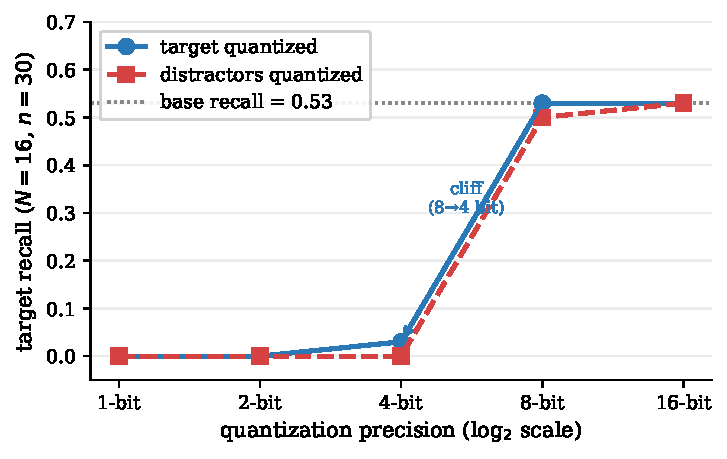
\includegraphics[width=0.62\linewidth]{nfig_quant.pdf}
  \caption{Write-quantization is not a graceful lever. Lowering a single item's
  write precision either does nothing ($\ge 8$ bits) or collapses recall
  ($\le 4$ bits); quantizing distractors to free capacity instead destroys the
  target, evidencing the absence of per-item slots.}
  \label{fig:quant}
\end{figure}

\begin{table}[t]
\centering
\caption{Write-precision quantization at $N{=}16$. This probe uses an
independent self-contained MQAR harness whose full-precision base recall is
$0.53$ (cf.\ $0.77$ in Table~\ref{tab:main}); we read the \emph{shape} of the
precision curve, not absolute values. Neither targeting nor reallocation
behaves like bit allocation in a slotted cache.}
\label{tab:quant}
\begin{tabular}{lccccc}
\toprule
Quantize & 16-bit & 8-bit & 4-bit & 2-bit & 1-bit \\
\midrule
target      & 0.53 & 0.53 & 0.03 & 0.00 & 0.00 \\
distractors & 0.53 & 0.50 & 0.00 & 0.00 & 0.00 \\
\bottomrule
\end{tabular}
\end{table}

The negative result is still informative. Because the state is a superposition with
no random-access slots, lowering one item's write precision either does nothing
($\ge 8$-bit) or injects noise the whole sequence shares ($\le 4$-bit). There is
no per-item bit budget to reallocate. The importance-allocation principle thus
transfers to Mamba \emph{only} through retention (Section~\ref{sec:circuit}), not
through quantization. This is a concrete boundary on the KV-cache analogy and an
empirical instance of the ``no slots'' property that distinguishes
continuous-state memory from a discrete cache.

\section{Limitations and Scope}\label{sec:limits}
\textbf{Single model:} all positive results are for Mamba-790m.
Scale checks in both directions fail to replicate the circuit.
\emph{Larger (1.4b):} all layer-band $\Delta \le 0$ despite ample headroom --- no
positive circuit at a comparable pressure regime.
\emph{Smaller (130m):} a weak effect exists at L13--16
($\Delta{+}0.06$, vs.\ $+0.17$ for 790m) but at an anomalous relative depth
($57$--$70\%$ vs.\ $40$--$47\%$), with PPL decreasing rather than increasing
($\times 0.95$), suggesting different layer dynamics at this scale.
The L16--23 circuit appears to be a property specific to the 790m scale; we do not
claim a universal depth or mechanism.
\textbf{Synthetic task:} effects are robust on random-token MQAR but fragile on
natural-language multi-fact recall, where the intervention can hurt.
\textbf{Graded priority is real but weak:} a de-confounded experiment
(Experiment~E) confirms that other-gain level causally controls retention independent of
write position --- P1 ($g{=}0.7$) achieves $0.13$ vs.\ P3 ($g{=}1.0$) at $0.00$
after marginalizing over pair positions (Table~\ref{tab:graded}). However, the
original strong confounded result (P1$=0.53$) was largely a write-position artifact,
and the de-confounded effect is modest in absolute terms. The SSM shared-decay
constraint ($\Delta>0\Rightarrow\bar{A}<1$, same trajectory for all pairs) limits
item-selective allocation, consistent with Section~\ref{sec:boundary}; we do not
claim robust multi-level allocation.

\section{Related Work}
\paragraph{SSM capacity.}
\citet{jelassi2024} establish the copying/capacity limit; work on primacy/recency
documents the default decay policy. We add a controllability result on top of the
capacity picture.
\paragraph{KV-cache compression.}
KIVI, KVQuant, ZipCache and rotation-based quantizers \citep{turboquant} realize
importance-aware bit allocation on slotted caches; we ask whether the principle
survives the move to a slotless continuous state, and find it survives as
retention but not as quantization.
\paragraph{Recall and the ``what to keep'' frontier.}
Prompting methods such as Just Read Twice \citep{jrt} and architectures such as
Based, DeltaNet and Titans \citep{titans} target the same problem, mostly by
training new architectures or memory modules; ours is a training-free,
frozen-base alternative. We directly compare against JRT (Experiment~D,
Table~\ref{tab:jrt}): JRT achieves higher recall ($+0.47$ at $N{=}32$) at
$\times 1.97$ sequence overhead; PCR provides a zero-overhead alternative
($+0.17$, $\times 1.00$), identifying a recall-vs-cost operating-point split.
\paragraph{Mechanistic interpretability.}
Localizing a behavior to a contiguous layer band parallels circuit-style findings
in Transformers; ours is, to our knowledge, an early such localization of a
\emph{controllable} memory mechanism in a pretrained SSM.

\section{Conclusion and Future Work}
A pretrained Mamba's associative recall is, in part, a controllable property of a
specific middle-layer band, not a fixed ceiling. A surgical, training-free
intervention on layers~16--23 --- with a 4-layer minimal core at L19--22 that
matches the 8-layer recall ($0.70$ vs.\ $0.67$; confirmed equivalent at $n{=}150$)
and is both sufficient and necessary (Experiment~G) --- recovers
recall at negligible language-modeling cost. The importance-aware compression principle transfers to continuous state
through retention but not through quantization. Our proposed next step is to
remove the oracle: a small \emph{question-conditioned, auto-localizing} controller
trained on a frozen base, evaluated against Belady-MIN retention efficiency under
streaming queries, toward a training-free improvement of the recall--capacity
frontier of pretrained SSMs.

\begin{thebibliography}{9}
\small
\bibitem[Jelassi et al.(2024)]{jelassi2024} S.~Jelassi, D.~Brandfonbrener, S.~Kakade, and E.~Malach. Repeat After Me: Transformers are Better than SSMs at Copying. In \emph{ICML}, 2024.
\bibitem[Liu et al.(2024)]{kivi} Z.~Liu et al. KIVI: A Tuning-Free Asymmetric 2bit Quantization for KV Cache. In \emph{ICML}, 2024.
\bibitem[Hooper et al.(2024)]{kvquant} C.~Hooper et al. KVQuant: Towards 10M Context Length LLM Inference. In \emph{NeurIPS}, 2024.
\bibitem[He et al.(2024)]{zipcache} Y.~He et al. ZipCache: Accurate and Efficient KV Cache Quantization with Salient Token Identification. In \emph{NeurIPS}, 2024.
\bibitem[Zandieh et al.(2026)]{turboquant} A.~Zandieh et al. TurboQuant: Online Vector Quantization with Near-Optimal Distortion Rate. In \emph{ICLR}, 2026.
\bibitem[Arora et al.(2024)]{jrt} S.~Arora et al. Just Read Twice: Closing the Recall Gap for Recurrent Language Models. \emph{arXiv:2407.05483}, 2024.
\bibitem[Behrouz et al.(2024)]{titans} A.~Behrouz, P.~Zhong, and V.~Mirrokni. Titans: Learning to Memorize at Test Time. \emph{arXiv}, 2024.
\bibitem[Gu and Dao(2023)]{mamba} A.~Gu and T.~Dao. Mamba: Linear-Time Sequence Modeling with Selective State Spaces. \emph{arXiv:2312.00752}, 2023.
\end{thebibliography}

\end{document}
